% !TEX program = xelatex
\documentclass[10pt,a4paper]{article}

% ======================== 基础包 ========================
\usepackage[top=0.55cm,bottom=0.5cm,left=1.0cm,right=1.0cm]{geometry}
\usepackage{ctex}
\usepackage{titlesec}
\usepackage{enumitem}
\usepackage{xcolor}
\usepackage{graphicx}
\usepackage{hyperref}
\usepackage{fontawesome5}
\usepackage{tikz}

% ======================== 颜色定义 ========================
\definecolor{primary}{HTML}{2B4C7E}
\definecolor{darktext}{HTML}{2D2D2D}
\definecolor{graytext}{HTML}{666666}
\definecolor{rulecolor}{HTML}{B0B0B0}
\definecolor{photoframe}{HTML}{8C99AD}

% ======================== 超链接 ========================
\hypersetup{
    colorlinks=true, linkcolor=primary, urlcolor=primary,
    pdfauthor={徐其栋}, pdftitle={徐其栋 - 求职简历}
}

% ======================== 字体设置 ========================
\setCJKmainfont{SimHei}[BoldFont=SimHei]
\setmainfont{Segoe UI}[BoldFont=Segoe UI Bold]

% ======================== 段落和间距 ========================
\setlength{\parindent}{0pt}
\setlength{\parskip}{0pt}
\pagestyle{empty}

% ======================== 标题样式 ========================
\titleformat{\section}
    {\large\bfseries\color{primary}}
    {}{0em}{}
    [\vspace{-0.5em}{\color{rulecolor}\rule{\textwidth}{0.6pt}}\vspace{-0.2em}]
\titlespacing*{\section}{0pt}{0.35em}{0.2em}

% ======================== 自定义命令 ========================
\newcommand{\projectblock}[3]{%
    {\bfseries\color{darktext}#1}\hfill{\color{graytext}#2}\\%
    {\small\color{graytext}#3}%
    \vspace{0.15em}%
}

% ======================== 文档开始 ========================
\begin{document}

% ======================== 头部：左信息 + 右照片 ========================
\begin{minipage}[b]{0.72\textwidth}
    {\fontsize{25}{30}\selectfont\bfseries\color{primary}徐其栋}\\[16pt]
    {\small\color{primary}%
    \faBirthdayCake\hspace{0.35em}23 岁\hspace{0.75em}{\color{rulecolor}·}\hspace{0.75em}%
    \faUserGraduate\hspace{0.35em}2026 届应届生\hspace{0.75em}{\color{rulecolor}·}\hspace{0.75em}%
    \faYenSign\hspace{0.35em}期望薪资 5K--8K}\\[9pt]
    {\small\color{graytext}%
    \faPhone\hspace{0.35em}17268891140\hspace{0.75em}{\color{rulecolor}/}\hspace{0.75em}%
    \faEnvelope\hspace{0.35em}\href{mailto:xqd922@outlook.com}{xqd922@outlook.com}\hspace{0.75em}{\color{rulecolor}/}\hspace{0.75em}%
    \faGlobe\hspace{0.35em}\href{https://1001.pp.ua}{1001.pp.ua}}
\end{minipage}\hfill
\begin{minipage}[b]{0.25\textwidth}
    \raggedleft
    {\setlength{\fboxsep}{0pt}\setlength{\fboxrule}{0.7pt}%
     \color{photoframe}\fbox{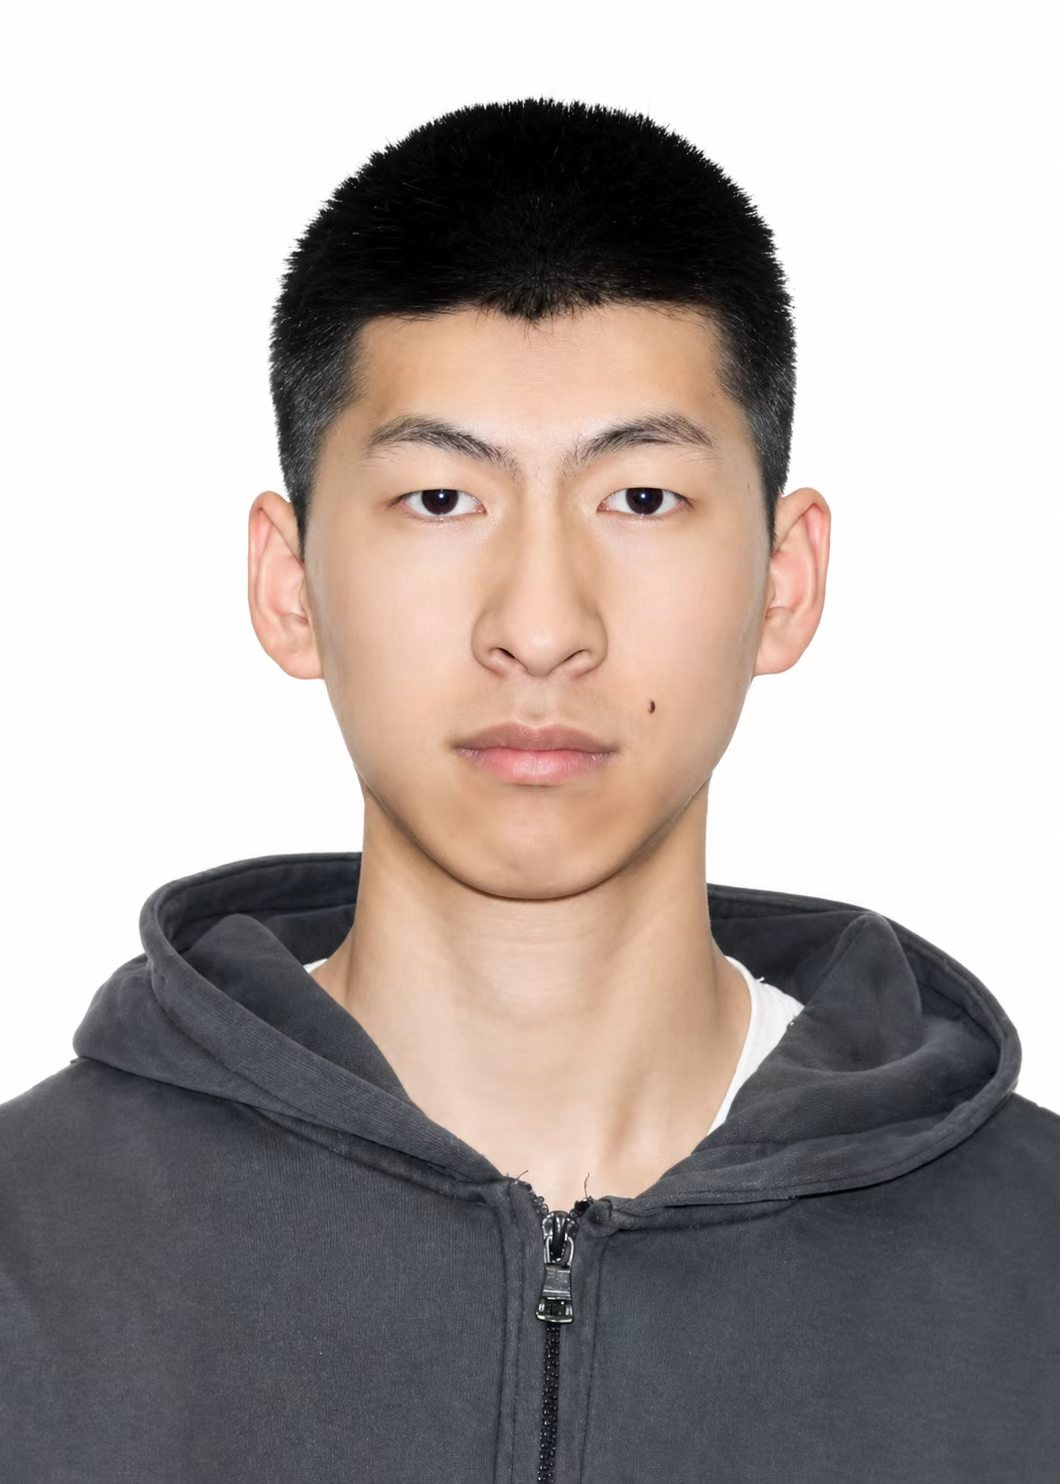
\includegraphics[height=3.6cm]{photo.jpg}}}
\end{minipage}

\vspace{2pt}
{\color{primary}\rule{\textwidth}{1.1pt}}

% ======================== 教育背景 ========================
\section{\faGraduationCap\hspace{0.4em}教育背景}

{\bfseries 滇西科技师范学院}\hfill{\bfseries 物联网工程\hspace{0.3em}|\hspace{0.3em}本科}

{\color{graytext} 2022.09 -- 2026.07}

\vspace{0.2em}

{\color{darktext}\textbf{主修课程：}C 语言、单片机原理、嵌入式技术、计算机网络、传感器原理、数字电子技术、模拟电子技术}

% ======================== 专业技能 ========================
\section{\faCogs\hspace{0.4em}专业技能}

{\bfseries\color{primary}嵌入式 / 物联网：}\hspace{0.3em}{\color{darktext}STM32、ESP32、外设驱动调试、I2C、UART、PWM、MQTT、EMQX、蓝牙、Wi-Fi、FreeRTOS}

\vspace{2pt}

{\bfseries\color{primary}编程与数据库：}\hspace{0.3em}{\color{darktext}C 语言、C++、Python、C\#、Qt、MySQL}

\vspace{2pt}

{\bfseries\color{primary}开发工具：}\hspace{0.3em}{\color{darktext}Keil MDK、Visual Studio、Git、Linux、嘉立创 EDA、示波器 / 逻辑分析仪}

% ======================== 实习经历 ========================
\section{\faBriefcase\hspace{0.4em}实习经历}

{\bfseries 云南航天工程物探检测股份有限公司}\hfill{\color{graytext}嵌入式软件开发实习生\hspace{0.3em}·\hspace{0.3em}2025.08 -- 2025.12}

\vspace{2pt}

\begin{itemize}[leftmargin=1.5em, itemsep=1pt, parsep=0pt, topsep=2pt]
    \item \textbf{底层驱动与采集节点开发}：基于 C/C++ 参与隧道、桥梁、路面工程检测设备的底层软件开发，独立完成采集节点程序设计与传感器数据的采集、滤波与处理。
    \item \textbf{数据显示与人机交互}：开发检测数据的实时显示与人机交互功能，结合现场作业流程优化设备操作逻辑，提升检测作业效率。
    \item \textbf{系统联调与版本管理}：排查并修复程序 Bug 与设备通信异常，承担软件联调、性能优化与版本迭代，使用 Git 进行代码版本管理与团队协作。
\end{itemize}

\vspace{0.2em}

% ======================== 项目经历 ========================
\section{\faProjectDiagram\hspace{0.4em}项目经历}

\projectblock{四足物联网机器狗控制系统}{2025.03 -- 2025.04}{技术栈：STM32F407ZE\hspace{0.3em}|\hspace{0.3em}PCA9685\hspace{0.3em}|\hspace{0.3em}ESP32\hspace{0.3em}|\hspace{0.3em}MPU6050\hspace{0.3em}|\hspace{0.3em}WS2812\hspace{0.3em}|\hspace{0.3em}I2C\hspace{0.3em}|\hspace{0.3em}UART\hspace{0.3em}|\hspace{0.3em}运动学逆解}

\begin{itemize}[leftmargin=1.5em, itemsep=1pt, parsep=0pt, topsep=2pt]
    \item \textbf{四足运动控制}：以 STM32F407ZE（168MHz Cortex-M4）为主控，通过 PCA9685 经 I2C 扩展 16 路 12 位 PWM 驱动 8 路舵机（四腿 $\times$ 2 关节），实现前进、后退、转向、站立等 9 类步态动作。
    \item \textbf{运动学逆解（核心难点）}：自主推导运动学逆解算法，基于余弦定理由足尖目标坐标 $(x, y)$ 反解大小腿关节角度，加入目标点可达性判断与 0\textdegree--180\textdegree{} 角度限幅；结合 1\textdegree{} 步进插值实现舵机平滑过渡，消除机械冲击与抖动。
    \item \textbf{姿态感知与多模交互}：MPU6050 经 I2C 读取六轴姿态实现倾倒检测与姿态反馈；蓝牙（USART2）支持网页远程遥控、ESP32（UART4）实现语音控制，WS2812 灯效实时反馈系统运行状态。
\end{itemize}

\vspace{0.15em}

\projectblock{STM32 智能交互台灯控制系统}{2026.03 -- 2026.05}{技术栈：STM32F103C8T6\hspace{0.3em}|\hspace{0.3em}自绘PCB\hspace{0.3em}|\hspace{0.3em}ADC光敏\hspace{0.3em}|\hspace{0.3em}HC-SR04\hspace{0.3em}|\hspace{0.3em}红外感应\hspace{0.3em}|\hspace{0.3em}USART2/3\hspace{0.3em}|\hspace{0.3em}TIM2 PWM\hspace{0.3em}|\hspace{0.3em}OLED}

\begin{itemize}[leftmargin=1.5em, itemsep=1pt, parsep=0pt, topsep=2pt]
    \item \textbf{硬件设计与驱动联调}：独立设计并自绘控制板 PCB，基于 STM32F103C8T6 完成按键、蜂鸣器、OLED、光敏、红外、超声波、蓝牙 / 语音等多模块的驱动开发与硬件联调。
    \item \textbf{多模式智能控制}：实现自动 / 手动 / 蓝牙 / 语音四种控制模式；ADC 采集环境光并经 TIM2 PWM 分档调光，融合红外在位检测与 HC-SR04 超声波测距实现无人自动关灯与近距离报警。
    \item \textbf{人机交互与远程控制}：OLED 实时显示光照档位与工作模式，USART2/3 接入蓝牙与语音模块实现远程调节与语音控制，独立完成从硬件设计到固件开发的软硬件一体化闭环。
\end{itemize}

\vspace{0.15em}

% ======================== 个人评价 ========================
\section{\faUser\hspace{0.4em}个人评价}

具备 \textbf{多个嵌入式项目实战经验}，能 \textbf{独立完成硬件选型、PCB 设计、驱动调试与运动控制算法开发}；熟悉 \textbf{MQTT 物联网通信与端云数据链路}，可胜任嵌入式软件开发岗位。

\end{document}
